

\documentclass[11pt]{article}
\usepackage{acl2011}
\usepackage[utf8]{inputenc}
\usepackage{linguex}
\usepackage{latexsym}  
\usepackage{graphicx}
\usepackage{multirow}
\usepackage{verbatim}
\usepackage{array}
\usepackage{subfigure}
\usepackage{hyperref}
\usepackage{amsmath}
\usepackage{qtree}
\usepackage{textcomp}
\usepackage{todonotes}
\usepackage{placeins}


%\usepackage{gb4e}

%\usepackage{gb4e}


% \usepackage{xcolor}
% \definecolor{dark-red}{rgb}{0.4,0.15,0.15}
% \definecolor{dark-blue}{rgb}{0.15,0.15,0.4}
% \definecolor{medium-blue}{rgb}{0,0,0.5}
% \hypersetup{
%     colorlinks, linkcolor={dark-red},
%     citecolor={dark-blue}, urlcolor={medium-blue}}
\title{Named Entity Recognition as Structured Prediction}

% \author{Joachim Daiber \\
%   %Affiliation / Address line 1 \\
%  
%   {\tt email@domain} \\\And
%   Carmen Klaussner \\
%   %Affiliation / Address line 1 \\
% 
%   {\tt carmen@wordsmith.de} \\
%   }
% 
% \date{today}


\author{Joachim Daiber \\
  University of Groningen \\
  2397331\\
  %Affiliation / Address line 3 \\
  {\tt jodaiber@gmx.de} \\\And
  Carmen Klaussner \\
  University of Groningen \\
  2401541\\
  %Affiliation / Address line 3 \\
  {\tt Carmen@wordsmith.de} \\}

\date{}

\DeclareMathOperator*{\argmax}{arg\,max}

\newcommand{\namedentity}{Named Entity} 
\newcommand{\Oo}{\texttt O} 


\begin{document}
\maketitle

\begin{abstract}
In this paper, we apply the method of structure prediction to the Named Entity Recognition (NER) information extraction task. 
We illustrate a number of issues relevant to the NER task, describe our implementation and compare it to state-of-the art methods.
%We use a structured version of the Perceptron algorithm with averaging and Viterbi decoding.
\end{abstract}


\section{Application: Named Entity Recognition}

Named Entity Recognition (NER) is a fundamental task for wide variety of natural language processing applications, including information retrieval and question answering
and thus provides a general basis for semantic analysis of texts \cite{Chen:2010:UDB:1870457.1870473}.

NER is an information extraction task and has first been introduced as part of the 6th MUC (Sixth Message Understanding Conference)
that was focusing on the extraction of structured information from unstructured text, such as company names from newspaper articles \cite{nadeau2007survey}.
The most prominent types of Named Entities are generally known under the name ENAMEX and are comprised of \texttt{Person Names}, \texttt{Organisations} and \texttt{Locations}.
An additional type \texttt{Miscellaneous} captures names outside the classic ENAMEX types.
Apart from the above, there is also the TIMEX type, which covers date and time expressions and NUMEX for monetary values and percentages.
Table~\ref{table:NETypes} provides an overview of the different Named Entity (NE) types.

\begin{table}[h!]
\scriptsize
\begin{tabular}{ l l }

\bf Named Entity Type & \bf Example \\
\hline 
Person Names & Greta Garbo, John, Mary \\
Organisations& Benetton, Coca-Cola Gmbh\\
Locations&  Paris, Australia, Bristol\\
Miscellaneous& World Cup 2014, Italien\\
 Date Expression& 01-02-2012, January, 6th, 1998 \\
Time Expression & 10 p.m.\\
Monetary Value &  \$15, \textsterling 100    \\
Percent &   30\% \\
\end{tabular}
\caption{Named Entity Examples}
\label{table:NETypes}
\end{table}


In considering Named Entities, it is important not to confuse them with non-specific entities. % reformulate
The difference lies in the reference of the entity. A Named Entity refers to a specific, unique person/time/location, whereas
\emph{normal} entities can refer to multiple events, such as the time expression: \emph{In June}, which could refer to any year.
Also, there could be a reference to a person, as in: \emph{the prof}, which in itself is not a \namedentity.
%However, it would be a deictic reference and point back to the mention of a real \namedentity, as in the following coreference chain: \\

%\ex. $ Prof.\; Bateman \Rightarrow he \Rightarrow the \; prof$ \label{cor}\\
A Named Entity can consist of more than one syntactic type. Syntactic types feature in syntactic rules that define how sentences can be build.
Typical high-level rules include:

\ex. $\text{S} \rightarrow \text{NP}\  \text{VP} $ \footnote{ A sentence (S) breaks down into a noun phrase (NP) and a verb phrase (VP)} \\
$ \text{VP} \rightarrow \text{V}\  (\text{NP})$ \footnote{ A verb phrase (VP) consists of a verb followed by an optional NP} 

Thus, sentences are often represented as syntactic trees that model the dependencies among the types.
The overall type for a Named Entity is usually a noun phrase (NP), which can be both simple and complex, meaning it can consist of a only a noun phrase or 
also additional other syntactic types, such as prepositional phrases (PP), that consist of a preposition and a noun phrase. 
%%%%%%%%%%%%%%%%%%%%%%%%%%%%%%%%%%%%%%%%%%% - can be left out if not enough space/too detailed
It is therefore a recursive definition and in theory, noun phrases can grow infinitely big, as shown by the recursive rules in example~\ref{recRules}.  % 

\ex. $ \text{NP} \rightarrow \text{NP} \  \text{PP}$ \\ \label{recRules}
     $ \text{PP} \rightarrow \text{P} \  \text{NP}$ 
 %%%%%%%%%%%%%%%%%%%%%%%%%%%%%%%%%%%%%%%%%%%%%%%%%%%%%%%%%%%%%%
 

% \ex. The Bank of Scotland is in the brown building with the brown bricks on its roof... \label{PPrec}
% 
% The PP \emph{of Scotland} is semantically defining for the noun \emph{bank}, whereas \emph{with the brown bricks on its roof} 
% just adds to the description of \emph{brown building}.

\subsection{Issues in Named Entity Recognition}

In order to illustrate linguistically motivated problems in NER, we consider the following problem, which is addressed in our model by a feature.

We distinguish between PP-complements and PP-modifiers. Complements are non-optional elements of the noun phrase as they are
inherent to the meaning of the entity. Modifiers only add to the description and are optional.
The syntactic trees in \ref{fig:bos} and \ref{fig:nirvana} show two examples for a complex noun phrase containing Named Entites.
\emph{N'} signals an intermediate state in the syntactic tree where modifiers can be joined.
In \ref{fig:bos}, (\emph{Bank of Scotland}), the PP \emph{of Scotland} is attached directly; it is central to the meaning, 
whereas in \ref{fig:nirvana} both \emph{Kurt Cobain} and \emph{Nirvana} constitute own concepts and are joined at a later level to express this distance.
Thus, in Named Entity Recognition, we want to be able to capture types of the first example as a single \namedentity~(\emph{Bank of Scotland}), 
but treat the second example as two separate Named Entities (\emph{Kurt Cobain} and \emph{Nirvana}).

% \begin{figure}
% \begin{enumerate}
% \item \parbox[t]{2.4in}{~\Tree  
%    [.NP [ [.DT the ] [.N\1 [.N Bank ] [.PP [.P of ] [.NP Scotland ] ] ] ] ] } \label{bos}
% \item \parbox[t]{2in}{~\Tree 
%    [.NP  [.N\1 [.N\1  \qroof{Kurt Cobain}.N  ]  [.PP [.P of ] [.N\1 [.N\1 [.N Nirvana ] ] ] ] ] ]  } \label{Nirvana}
% \end{enumerate} \label{Tree}
% \end{figure}

\begin{figure}
\Tree  
   [.NP [ [.DT the ] [.N\1 [.N Bank ] [.PP [.P of ] [.NP Scotland ] ] ] ] ] 

\caption{\namedentity: Complement Meaning}
\label{fig:bos}
\end{figure}


\begin{figure}
\Tree 
   [.NP  [.N\1 [.N\1  \qroof{Kurt Cobain}.N  ]  [.PP [.P of ] [.N\1 [.N\1 [.N Nirvana ] ] ] ] ] ]  

\caption{\namedentity: Reference Meaning}
\label{fig:nirvana}
\end{figure}

Generally, one of the most common challenges for NER is the issue of ambiguity, in particular \emph{Polysemy} \cite{nadeau2007survey}. %and \emph{Metonymy} insert with other section
Polysemy refers to the property of a lexical representation (\~ word) having more than one possible meaning. Polysemy can become an issue for NER when this lexical representation 
points to two different Named Entity types.
This is quite frequent with \texttt{Person Names} and \texttt{Locations}, since many people are named after cities and vice versa, for example \emph{Paris} or \emph{Georgia}. 
Often, context is not sufficient to disambiguate such names as in example~\ref{ex:Georgia}.

\ex. \emph{Georgia is beautiful.} \label{ex:Georgia}

% So lange ich nicht sicher weiß, wie damit in den CONLL Annotationen umgegangen wird, find ich das ein bisschen gefährlich...
%\emph{Metonymy} is the relationship of a part-whole relation between two items.
%It is frequently employed in literary texts and news data (which is often used in NER), where one item is substituted for another. 
%Example \ref{ex:Lon} shows an instance of a \emph{whole-part}, where \emph{London} probably stands for the smaller 'item': \textbf{Goverment in London}. 

%\ex. \emph{\textbf{London} decided to increase the 1200 military personnel involved in Olympic security.} %\label{ex:Lon}


\subsection{Approaches to NER}

Initially, rule-based methods were prevailing in the extraction of Named Entities. These methods make use of the underlying rules governing a language.
This approach, however, is very high in maintenance and requires extensive work by experts, such as computational linguists \cite{nadeau2007survey}.
The results achieved were reasonably good, but presented some flaws since constructed rules are dependent on the language and the domain and are not readily portable. 
This is the reason why nowadays machine learning methods are more attractive for this task as they offer more adaptability. 

For ML, supervised learning is the most common method applied in NER.
Although there are unsupervised methods, they cannot currently compete with supervised applications.
For the CoNLL shared task in 2002 \cite{tksintro}, 12 systems participated in the challenge and introduced a wide variety of approaches to the Named Entity task.
The most successful system used AdaBoost applied to fixed-depth decision trees. Special attention was given to a variety of input features, some which were also
particularly adapted for each language. I achieved an F-score of 81.39 on the Spanish test set and 77.05 on Dutch.
The second best system \cite{Florian:2002:NER:1118853.1118863} employed three stacked
learners (transformation-based learning for obtaining base-level non-typed Named Entites, sparse network of winnows (Snow) for improving the quality of these entities 
and the forward-backward algorithm for finding the categories for the Named Entites), where the combination of these three algorithms substantially outperformed 
any subset of them and yielded an F-score of 79.05 on the Spanish test set and 74.99 on Dutch.
Among the most prominent algorithms in NER are maximum entropy models, whose benefit in regard to this task became most apparent in CoNLL 2003. 
Five of the sixteen systems that participated used maximum entropy models, which appear to be a suitable choice for the NER task, 
since systems using this approach were ranked among the highest results in English and in German \cite{TjongKimSang:2003:ICS:1119176.1119195}.
The best system in both German and English \cite{Florian:2003:NER:1119176.1119201} used a combination of classifiers: a robust linear classifier, 
a maximum entropy classifier, a transformation-based learner, and a hidden Markov model. The models were connected through a linear interpolation 
of the classifiers’ % combination scheme
class probability distribution. Particular importance was also assigned to creating a rich feature space, also including a gazetteer feature. 
This system achieved a F-score of 88.76\% on the English test set and 72.41\% on the German one.
Another, more recent approach involved the use of Deep Belief Nets (DBN) for NER in Chinese \cite{Chen:2010:UDB:1870457.1870473}.
Due to the language's special characteristics of lacking boundary information, character-based methods are generally given preference over word-based methods.
In their application for NER, DBN  was used to automatically discover the complicated composite effects of the characters to the NE categories from the input data. 
The paper reports DBN's strong representative power in regard to detection of more complicated and efficient features. With a precision of 91.45\%,
it achieved better performance than both a SVM and a BP neural networks.

\subsection{CoNLL Data and Baseline Performance}
The training and test data for Spanish and Dutch was taken from the CoNLL Shared Task 2002 \cite{tksintro} and 
the CoNLL Shared Task 2003 \cite{TjongKimSang:2003:ICS:1119176.1119195} provided the data for English and German.
%The ConNLL shared tasks are organized challenges, where the organisers propose a task and provide the participants with the
%training and test data. 
%In 2002 and 2003, the task was Named Entity Recognition. 
In 2002 and 2003 CoNLL shared tasks were on Named Entity Recognition. The baseline system was constructed by first determining
on the most frequent Named Entity class C in the training data and then labeling all occurrences of a Named Entity found in the test data with class C regardless of context. 
Any Named Entities that did not occur in the training data were also not assigned any class in the test data.
Given that a phrase was part of more than one entity, the system would choose the longest one \cite{TjongKimSang:2003:ICS:1119176.1119195}.
Table~\ref{table:Base} shows the baselines for the four different languages.  
The data was annotated with part-of-speech tags and Named-Entity tags, as well as BIO-tags that indicate the position of a token in the current Named Entity. %put in ``tokenized, chunked''
%Our approach is based on \cite{strlearn}, of the group that won the challenge for Spanish and Dutch in 2002. 


\begin{table}[h!]
\small
\begin{tabular}{|l|l|l|l|}
\hline
\bf Language & \bf Precision & \bf Recall & \bf $F_1$-measure \\ \hline
Spanish &             26.27\% & 56.48\% & 35.86\%        \\
Dutch  &             64.38\%  &45.19\%    & 53.10\%  \\
English &              71.91\%& 50.90\%  & 59.61 $\pm$ 1.2\%\\
German &      31.86\%  & 28.89\% & 30.30  $\pm$ 1.3\% \\
\hline
\end{tabular}
\caption{Named Entity Recognition baselines.}
\label{table:Base}
\end{table}



\section{Implementation}
In this section, we describe our implementation, the learning and decoding algorithm and the features that were used.

\subsection{Structured Prediction}
Structured Prediction \cite{Taskar:2005:LSP:1102351.1102464} is an approach to supervised learning that is often used in natural language processing. 
Assuming our goal is to learn a function ${ \boldsymbol{f}\colon \mathcal{X}\to\mathcal{Y} }$, in Structured Prediction, we assume that $y \in \mathcal{Y}$ 
is not atomic (e.g.\ binary prediction), but that the prediction is a structure (e.g.\ a syntactic tree for a sentence or a sequence of part-of-speech tags). 

The structured prediction approach we follow has advantages over traditional approaches like hidden Markov models. While a hidden Markov model can model interactions 
between labels as transition probabilities, it is restricted to tokens and Maximum Likelihood learning. Another alternative would be to use a classifier for each 
token and then concatenate the results. However, this approach would not take into account label interactions. With Structured Prediction, we can use features and 
model label interactions at the same time.

\subsection{Learning and Decoding}

% problem external data / use Dbpedia - gazetteer
Our implementation for the languages English, German, Dutch and Spanish is trained and tested on the CoNLL 2003 and CoNLL 2002 data sets respectively. 


\begin{figure*}[ht]

\ex. \emph{The motor company 'Ford' was founded and incorporated  by Henry Ford.} \label{PredEx1a}
%The motor company 'Ford' was founded and incorporated  by Henry Ford on June, 16th 1903.
 
\exg. \textbf{x:} The motor company ' Ford ' was founded and incorporated by Henry Ford .\\
      \textbf{y:}  O   O      O     0 ORG  O  O     O     O       O        O PER   PER  O  \label{PredEx1b} \\
\caption{Input and predicted structure for the Named Entity Recognition task.}

\end{figure*}


As the predicted structure, we use the labels for every token in the full sentence. If a token is not a \namedentity, it is assigned the label \Oo.

Learning is implemented using the Structured Perceptron algorithm. To avoid overfitting, we average the parameters after the last iteration \cite{collins2002discriminative}. 
For finding the best sequence of labels for a sentence, we use a modified version of the Viterbi algorithm. The algorithm finds the sequence $\hat{y}$, such that:
\[
\hat{y} = \argmax_{\mathbf{y} \in \mathcal{Y}^{n}} \sum_{i=1}^{n}\mathbf{w} \cdot \boldsymbol{f}(\mathbf{x}, i, y_{i-1}, y_{i})
\]

This sequence can be computed efficiently in $ O( N^2 |\mathbf{x}| ) $ via dynamic programming. 
As a first step, the trellis has to be constructed, then we have to find the $ a \in \mathcal{Y}$ in the 
last column of the trellis with maximal score $\delta_n(a)$. From this, the sequence can be recovered via back-tracking trough the trellis. 
The score of the best sequence ending in $a$ is:
\[
\delta_i(a) = \max_{\mathbf{y} \in \mathcal{Y}^{n}, y_n = a} \sum_{j=1}^{n}{\mathbf{w} \cdot \boldsymbol{f}(\mathbf{x}, j, y_{j-1}, y_{j})}
\]

\noindent This function $\delta_i(a)$ can be defined recursively as:

\begin{align*}
\delta_1(a) &= \mathbf{w} \cdot \boldsymbol{f}(\mathbf{x}, 1, \emptyset, a) \\
\delta_i(a) &= \max_{b \in \mathcal{Y}} \delta_{i-1}(b) + \mathbf{w} \cdot \boldsymbol{f}(\mathbf{x}, i, b, a) \\
\end{align*}


\subsection{Features}
The features employed in the system can be divided into three categories: node, label and gazetteer features. 
We describe each of the three groups in the following.

\paragraph*{Node features}
Node features are features that only depend on the current token (node): the \emph{Token}, suffix and prefix and capitalisation.

Table~\ref{table:node} shows the various node features with an example respectively.

\begin{table}[h!]
\small
\begin{tabular}{ l l }
\bf Feature & \bf Example \\
\hline
Token &  \textbf{Amsterdam}\\
Suffix& Amster\textbf{dam}\\
Prefix&  \textbf{Mc}Cartney\\
Captitalized& \textbf{B}enetton\\
UPPERCASE &  \textbf{BENETTON}\\
Number patterns & 2005\\
POS tag &  Benetton \textbf{NNP}   \\
Lemma & produced $\Rightarrow$ produce \\

\end{tabular}


\caption{\normalsize Examples of node features.}
\label{table:node}
\end{table}

\paragraph*{Label Interaction Features}
These features model the interaction between the labels of adjacent tokens and take into account the most likely sequence. 
For the sequence ``Jack London went to New York'', the label combination of \emph{PER} and \emph{PER} as in \ref{seq1} is more likely than \emph{PER} and \emph{LOC} in \ref{seq2}.
%current token and last label for prepositions or possessive ’s

\exg. Jack London went to New York .\\
      PER   PER   O    O  LOC LOC  O \\\label{seq1}

\exg. Jack London went to New York . \\ 
      PER  LOC    O    O  LOC LOC O \\\label{seq2}
      
In addition, there is a prepositional phrase (PP) attachment feature, that registers the existence of an attachment, that would
result in a break of the sequence as in

\exg. Bank of Scotland . \\ 
      ORG   0    ORG   0  \\\label{seq3}
    

\paragraph*{Gazetteer Features}
A technique commonly used in Named Entity Recognition is the use of external lists of names of a specific type (gazetteer). 
In order to create gazetteer lists for more common Named Entities, we use a \emph{SPARQL} query  (Figure~\ref{fig:sparql}) 
to automatically retrieve entries from DBpedia for all required languages from a public SPARQL endpoint.

\begin{figure}
\begin{verbatim}
PREFIX d: <http://dbpedia.org/ontology/>
SELECT ?label
WHERE {
    ?entity rdf:type   d:CLASS.
    ?entity rdfs:label ?label.
    FILTER (lang(?label) = LANGUAGE)
}
\end{verbatim}
\caption{SPARQL query for retrieving names of the class \texttt{CLASS} from DBpedia.}
\label{fig:sparql}

\end{figure}

Given the lists of entities retrieved, we then mark the longest matches of known entities in the input using a directed acyclic word graph. 
The mention is annotated with a reference to its list of origin, which is then used as a feature in our model. With this approach, it is not 
necessary to manually map the lists to target labels and the model can learn the reliability of each list.


\subsection{Other Issues}

One of the issues that we needed to address was the case of headlines. Headlines, mainly in the English data, are often written entirely 
in uppercase letters. This is problematic because from most of the data, the model might learn that a word in all uppercase letters is 
indicative of an organisation (e.g.\ IBM, AIG, NYSE) and might thus mistake the tokens in headlines for organisations. 
We address this issue by converting all-uppercase headlines into their most likely original case (truecasing). 
To estimate the most likely case of a token from a monolingual corpus, we use the truecasing model from the 
Moses statistical machine translation system \cite{koehn2007moses}. 





\section{Experiments and Evaluation}

\subsection{Experiments}

\subsubsection{Influence of feature sets}

In the following, we show the influence of each of the three sets of features on the resulting accuracy.
\FloatBarrier
\begin{figure*}[t!]
\centering
 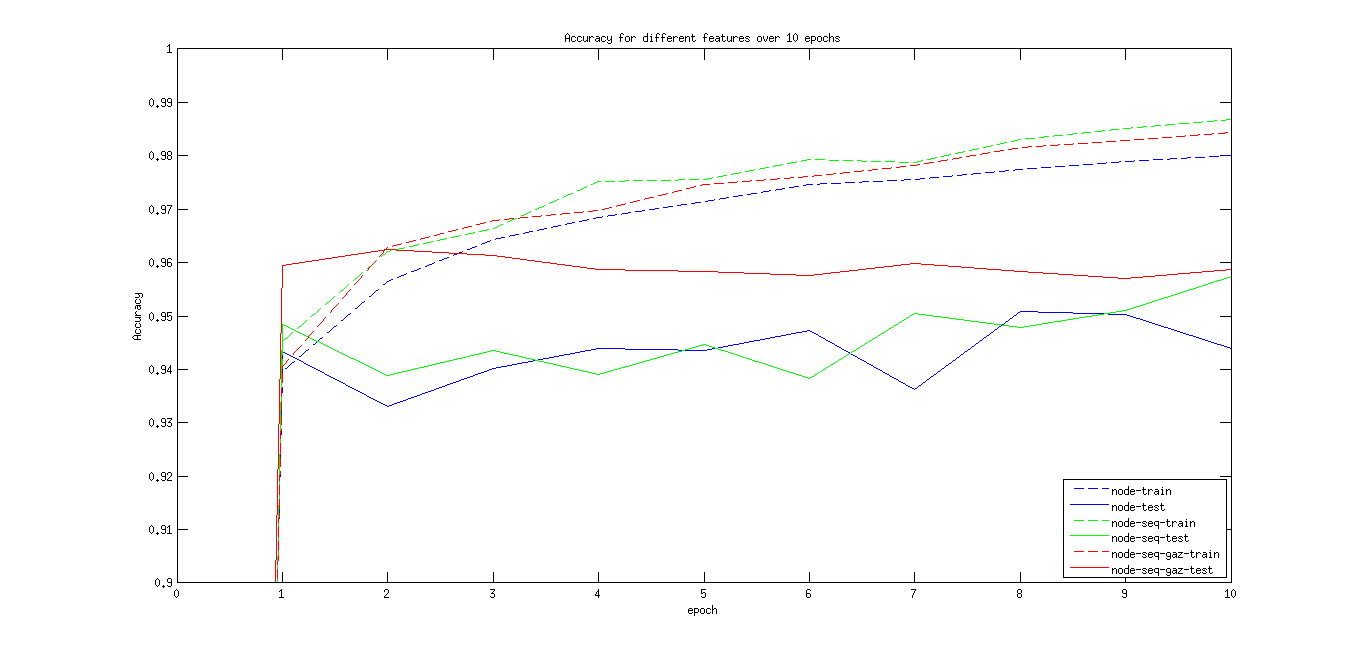
\includegraphics[scale=0.5]{Plot.png}
\end{figure*}


\subsubsection{Extending monolingual gazetteers}

The experiment above has shown that the gazetteer feature is beneficial for Dutch. In this experiment, we wanted to explore whether the 
gazetteer feature can be improved by extending the monolingual gazetteer with entries from other languages. For this, we compare the 
Dutch-only gazetteer with a gazetteer extended with English data.

% RESULTS FOR DUTCH


\subsection{Evaluation}

\begin{table*}[t]
\centering
\begin{tabular}{| l | l l l| l l l |}

\hline
\bf Language & \multicolumn{3}{c|}{ \bf Test A}&\multicolumn{3}{c|}{ \bf Test B}\\
             & Precision & Recall & $F_1$ & Precision & Recall & $F_1$ \\ \hline
Spanish &       &          &     &          &               & \\
Dutch  &         &          &     &          &               &   \\
English &        &          &     &          &               &       \\
German &      &          &       &          &             & \\
\hline
\end{tabular}
\caption{NER Structured Prediction Results }
\label{table:Results}
\end{table*}

For the evaluation of the system, we used the standard measure of \emph{precision} and \emph{recall} as shown below.
\begin{align*}
     precision =  \frac{  |\,gold\,\cap\,predicted\,| }{ |\,predicted\,| } \\
     recall = \frac{ |\,gold\,\cap\,predicted\,| }{ |\,gold\,| }
\end{align*}

Precision is the percentage of Named Entities found by the system that are correct. Recall is the percentage of Named Entities present in the corpus that were 
found by the system. A Named Entity is only deemed correct if it is an exact match for the corresponding data file. The general formula for the \emph{F-score} 
is shown below. Since we consider precision and recall as equally important, we use the $F_{1}$-score, which is the harmonic mean of precision and recall.
\begin{align*}
  F_{\beta} &=  (1+\beta^2)*\frac{precision *recall}{\beta^2* precision + recall}\\
  F_1       &= 2*\frac{precision *recall}{precision + recall}\\
\end{align*}





\section{Discussion}


\section{Future Work and Conclusion}

In this paper, we presented a \namedentity~Recognition system based on the concept of Structured Prediction. 
While the system does not achieve state-of-the-art performance on the CoNLL shared task, we believe that the results 
are reasonable for the following reasons: We are using a simple model, which has the advantage that the final application
will be fast and it is easily extendable. In contrast to the best systems in the CoNLL task, we also do not use ensemble 
learning methods and we use the same set of features for all languages, which enables simple extension of the system to additional languages.



\bibliographystyle{acl}
\bibliography{paper}

\end{document}
